\documentclass{bioinfo}
\copyrightyear{2015} \pubyear{2015}

\access{Advance Access Publication Date: Day Month Year}
\appnotes{Applications Note}

\begin{document}
\firstpage{1}

\subtitle{Sequence analysis}

\title[short Title]{Pathopred: Deep Convolutional Neural Network Predicting Pathogenicity of Non-Synonymous SNPs}
\author[Sample \textit{et~al}.]{Corresponding Author\,$^{\text{\sfb 1,}*}$, Co-Author\,$^{\text{\sfb 2}}$ and Co-Author\,$^{\text{\sfb 2,}*}$}
\address{Alexander Kvist $^{\text{\sf 1}}$Dep of Biochemistry and Biophysics and
  Science for Life Laboratory, Stockholm University, Solna, 171 21, Sweden. and \\
$Arne Elofsson^{\text{\sf 2}}$Dep of Biochemistry and Biophysics and
  Science for Life Laboratory, Stockholm University, Solna, 171 21, Sweden.}

\corresp{$^\ast$To whom correspondence should be addressed.}

\history{Received on XXXXX; revised on XXXXX; accepted on XXXXX}

\editor{Associate Editor: XXXXXXX}

\abstract{
\textbf{Summary:} Computational tools assist in interpreting
  SNPs which is important for the fast increasing amount of data generated
  from large scale sequencing projects of individual humans.  Here, we
  show that by using novel machine learning methods and incorporating
  sequence information, structural information, annotations and
  evolutionary conservation information, high prediction accuracy of
  harmful amino acid substitutions in human proteins can be
  achieved. The model PathoPred, a deep convolutional neural network, when trained on a VariBench benchmark
  dataset, achieves an improved prediction accuracy when predicting the probability of pathogenic substitutions compared to previous 
  individual methods, with an accuracy and MCC of 0.81 and 0.62 on an independent VariBench test
  set, respectively.\\
\textbf{Availability and Implementation:} The pathopred web server is
freely available at http://pathopred.bioinfo.se/. GPL licensed source code of
all pathopred specific programs and scripts can be obtained from
https://github.com/ElofssonLab/web\_pathopred/ \\
\textbf{Contact:} \href{arne@bioinfo.se}{arne@bioinfo.se}\\
\textbf{Supplementary information:} Supplementary data are available at \textit{Bioinformatics}
online.
}

\maketitle

\section{Introduction}

Single nucleotide polymorphisms (SNPs) make up much of the genetic
variation between humans. SNPs located in coding regions of the human
genome can cause amino acid changes in the final protein product of
genes. These non-synonymous single nucleotide polymorphisms (nsSNPs)
have been found to be linked to human disorders and are documented in
variation databases such as HGMD \citep{Stenson2003} and dbSNP
\citep{Sherry2001}. 

With an increasing amount of variants being found and documented as
sequencing technologies advance, computationally screening these
variants to find those valuable for further study is
important. Various computational tools exist to predict the effects of
variants. The effects that these tools attempt to predict range from
protein stability to the impact on transcription factor binding, to
the likelihood that a variant is involved in a disease. 

Machine learning methods such as PON-P2 \citep{Niroula2015} and
PolyPhen-2 \citep{Adzhubei2013} focus on the pathogenicity of nsSNPs,
that is, the probability that a variant is damaging or involved in
disease. These tools, and many other variant prediction tools like
them, will often employ features from sequence annotations, properties
of multiple sequence alignments (MSAs) constructed from searching for
homologs, or biochemical properties of amino acids. Certain predictors
such as PON-PS \citep{Niroula2017} will also attempt to predict the
severity of a disease phenotype arising from an amino acid
substitution.  

For the purpose of assessing the performance of computational predictors, benchmark databases have been created. One such database is VariBench \citep{Nair2013}, containing a number of datasets with data collected and organized from dbSNP and other sources. Amongst others, it contains a dataset for protein variant tolerance, used to train PON-P2 and a disease phenotype severity annotated dataset, used to train PON-PS.

Here, these datasets is used o train a novel predictor utilizing a
one-dimensional deep convolutional neural network to predict both the
pathogenicity as well as severity of variants in human proteins (for
details see supplementary material). 

\begin{methods}

\section{Materials and methods}

\subsection{Datasets}

The VariBench protein tolerance dataset used for training the Pathopred
binary pathogenicity predictor consists of a total of 28559 variants
from 7675 proteins, 14674 variants of which are classed as neutral,
and 13885 are classed as pathogenic. A second VariBench dataset was
used for training the Pathopred severity predictor
consists of a total of 2928 disease variants from 91 proteins, of
which 1028 variants are classes as mild, 501 as moderate, and 1399 as
severe. The datasets are separated into training sets and independent
test sets and are publicly available at the VariBench website (http://structure.bmc.lu.se/VariBench/).

\subsection{Features}

The input to pathopred consist of six feature vectors (see supporting
material).  

First, a BLAST search against the NCBI nr is used to find homologous
protein sequences. Two MSAs are constructed from these, one containing
sequences with sequence identity below 90\% to reference sequence, and
one containing 90\% sequence identity or above. The MSAs are
constructed using MAFFT.

From the mutation position, a window of 10 amino acids in each
direction is used to construct three of the feature vectors: The
frequencies of amino acids and gap characters in the MSA along with
the shannon entropy, the self-information \citep{Hurtado2018} for each
amino acid at a position, and the partial entropy \citep{Hurtado2018}
for each amino acid at a position.

The fourth feature vector is obtained from feeding the self-information
and partial entropy into a pre-trained deep convolutional neural
network \citep{Hurtado2018}, resulting in secondary structure,
relative surface area, and representations of protein backbone torsion
angles.

Finally, the amino acid sequence of the window is encoded as a one-hot
vector and included as a feature vector. Finally, the original and
reference amino acid are encoded as one-hot vectors, and appended to
this is a log-odds score calculated from the presence of GO terms
found in UniProtKB for the protein analyzed.

\subsection{Predictor}

The deep convolutional neural network consists of several layers of
one-dimensional blocks with a ResNet structure, ending in a
fully-connected layer of 128 neurons with a sigmoid output layer for
binary pathogenicity predictions, as well as for predicting between severe 
and non-severe pathogenic substitutions, see supplementary material. 
The predictors are built using the Keras library \citep{Chollet2017} and training is
guided by the Adam optimizer.

\end{methods}

\section{Results and discussion}

%These are the reported scores on the independent test set, from the study done in Niroula, and Pathopred scores
\begin{table}[!t]
\processtable{VariBench tolerance dataset: test set\label{Tab:01}} {\begin{tabular}{@{}llllllll@{}}\toprule 
Predictor & PPV & NPV & Sens & Spec & Acc & MCC & F1\\\midrule
Pathopred & 0.75 & 0.87 & 0.85 & 0.78 & 0.81 & 0.62\\
PON-P2 & 0.74 & 0.79 & 0.75 & 0.78 & 0.77 & 0.53\textsuperscript{a}\\
SNAP & 0.68 & 0.83 & 0.83 & 0.68 & 0.75 & 0.51\\
Condel & 0.71 & 0.79 & 0.76 & 0.73 & 0.75 & 0.49\\
PolyPhen-2 & 0.67 & 0.81 & 0.81 & 0.68 & 0.73 & 0.48\\
SIFT & 0.67 & 0.80 & 0.77 & 0.71 & 0.74 & 0.48\\
Provean & 0.67 & 0.78 & 0.74 & 0.72 & 0.73 & 0.46\\\botrule
\end{tabular}}{\textsuperscript{a}Performance with all variants included, as reported in \citep{Niroula2015}}
\end{table}

%TODO: should be a low-res TIF (re-generate from the saved data) -- also give it the correct pathopred name
\begin{figure}[!tpb]
\centerline{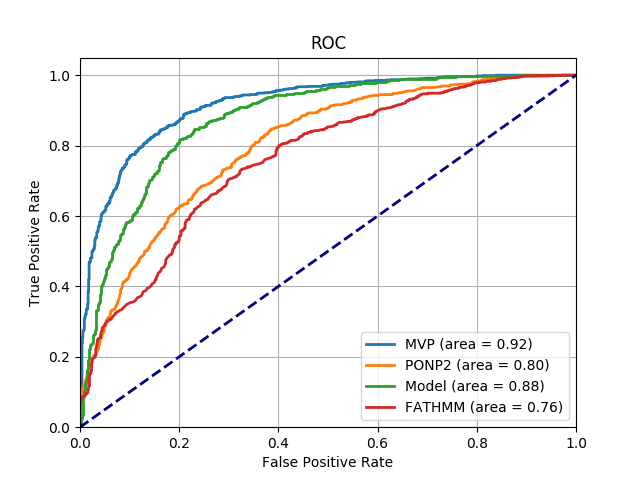
\includegraphics[scale=0.5]{varibench_tolerance_test_ROC.png}}
\caption{ROC curves and AUC of Pathopred, MVP, FATHMM, and PON-P2.}\label{fig:01}
\end{figure}

Results of the model on the independent VariBench test set for binary
pathogenicity prediction are presented in Table~\ref{Tab:01}, along
with several others predictors evaluated in
\citep{Niroula2015}. Pathopred improves on the other methods with an
MCC of 0.62. An independent evaluation with predictors found to have
high prediction accuracies in literature on the VariBench test set as
well as other test sets can be seen in Figure~\ref{fig:01}. The ROC
curves of Pathopred along with PON-P2 and two other predictors MVP
\citep{Qi2018}, an ensemble method, and FATHMM \citep{Shihab2013} are
presented. Pathopred shows a higher AUC than both PON-P2 and FATHMM
with an AUC of 0.88, but scores lower than MVP, which shows an AUC of
0.92. It should be noted that the MVP score in this comparison is
likely biased because of training data overlap with test data
\citep{Kvist2018}.

When predicting severity classes, distunguishing between non-severe
(mild and moderate) and severe on an independent VariBench test set,
Pathopred achieves an MCC of 0.21, as compared to PON-PS with an
identical MCC of 0.22 \citep{Niroula2017}, see supplementary
material.


In conclusion, while the severity prediction performs
similar to earlier best performing models, the binary predictions are
significantly improved.

\section*{Funding}

This work has been supported by the... Text Text  Text Text.%\vspace*{-12pt}

%\bibliographystyle{natbib}
%\bibliographystyle{achemnat}
%\bibliographystyle{plainnat}
%\bibliographystyle{abbrv}
%\bibliographystyle{bioinformatics}
%\bibliographystyle{plain}
%\bibliography{Document}

\begin{thebibliography}{}

\bibitem[Stenson, 2003]{Stenson2003}
Stenson, P. D., Ball, E. V., Mort, M., Phillips, A. D., Shiel, J. A., Thomas, N. S., ... and Cooper, D. N. (2003). Human gene mutation database (HGMD®): 2003 update. {\it Human mutation}, {\bf 21(6)}, 577-581.

\bibitem[Sherry, 2001]{Sherry2001}
Sherry, S. T., Ward, M. H., Kholodov, M., Baker, J., Phan, L., Smigielski, E. M., and Sirotkin, K. (2001). dbSNP: the NCBI database of genetic variation. {\it Nucleic acids research}, {\bf 29(1)}, 308-311.

\bibitem[Niroula, 2015]{Niroula2015}
Niroula, A., Urolagin, S., and Vihinen, M. (2015). PON-P2: prediction method for fast and reliable identification of harmful variants. {\it PloS one}, {\bf 10(2)}, e0117380.

\bibitem[Niroula, 2017]{Niroula2017}
Niroula, A., and Vihinen, M. (2017). Predicting severity of disease‐causing variants. {\it Human mutation}, {\bf 38(4)}, 357-364.

\bibitem[Nair, 2013]{Nair2013}
Nair, P. S., and Vihinen, M. (2013). VariBench: a benchmark database for variations. {\it Human mutation}, {\bf 34(1)}, 42-49.

\bibitem[Adzhubei, 2013]{Adzhubei2013}
Adzhubei, I., Jordan, D. M., and Sunyaev, S. R. (2013). Predicting functional effect of human missense mutations using PolyPhen‐2. {\it Current protocols in human genetics}, {\bf76(1)}, 7-20.

\bibitem[Kvist, 2018]{Kvist2018}
Kvist, A. (2018). Identifying pathogenic amino acid substitutions in human proteins using deep learning.

\bibitem[Hurtado, 2018]{Hurtado2018}
Hurtado, D. M., Uziela, K., and Elofsson, A. (2018). Deep transfer learning in the assessment of the quality of protein models. arXiv preprint arXiv:1804.06281.

\bibitem[Chollet, 2017]{Chollet2017}
Chollet, F. (2017). Keras (2015).

\bibitem[Qi, 2018]{Qi2018}
Qi, H., Chen, C., Zhang, H., Long, J. J., Chung, W. K., Guan, Y., and Shen, Y. (2018). MVP: predicting pathogenicity of missense variants by deep learning. bioRxiv, 259390.

\bibitem[Shihab, 2013]{Shihab2013}
Shihab, H. A., Gough, J., Cooper, D. N., Stenson, P. D., Barker, G. L., Edwards, K. J., ... and Gaunt, T. R. (2013). Predicting the functional, molecular, and phenotypic consequences of amino acid substitutions using hidden Markov models. {\it Human mutation}, {\bf 34(1)}, 57-65.


\end{thebibliography}
\end{document}
